\documentclass[12pt,a4paper]{article}
\usepackage[utf8]{vietnam}
\usepackage{amsmath,amssymb}
\usepackage{tabularx}
\usepackage{tikz}
\usetikzlibrary{calc,angles,quotes,arrows.meta,patterns}
\usepackage{xcolor}
\usepackage{enumitem}
\usepackage{fancyhdr}
\usepackage[top=1.2cm, bottom=1.2cm, left=1.5cm, right=1.5cm]{geometry}
\usepackage[dethi]{ex_test}
\SAOPTN{widthSA=2.6,heightSA=0.62}

\setlength{\headheight}{15pt}
\setlength{\parskip}{0pt}

% Dòng kẻ chấm mờ chuẩn viết tay
\newcommand{\dongke}[1]{%
  \begingroup%
  \setlength{\parskip}{0pt}%
  \baselineskip=18.5pt%
  \vspace{1.0mm}%
  \foreach \i in {1,...,#1}{%
    \noindent{\color{gray!60}\dotfill}\par%
  }%
  \vspace{0.6mm}%
  \endgroup%
}

\pagestyle{fancy}
\fancyhf{}
\rhead{\textit{Môn Toán 6 -- Đề số 2}}
\lhead{\textit{Bộ đề ôn tập Giữa học kì I}}
\cfoot{\thepage}

\begin{document}

% --- KHUNG TIÊU ĐỀ ĐỀ THI ---
\noindent
\begin{tabularx}{\linewidth}{X r}
\textbf{TRƯỜNG THCS: \dotfill} & \textbf{ĐỀ KIỂM TRA ĐỊNH KỲ GIỮA HỌC KỲ I} \\
\textbf{Họ và tên: \dotfill} & \textbf{NĂM HỌC 2026 -- 2027} \\
\textbf{Lớp: \dotfill \quad SBD: \dotfill} & \textbf{Môn: TOÁN 6} \\
\hline
\end{tabularx}
\vspace{2mm}

\begin{center}
  \textbf{\large ĐỀ ÔN TẬP GIỮA HỌC KỲ I -- ĐỀ SỐ 2}\\
  \textit{Thời gian làm bài: 90 phút (Không kể thời gian phát đề)}
\end{center}
\vspace{1mm}

% --- PHẦN I ---
\noindent\textbf{\large PHẦN I. CÂU TRẮC NGHIỆM NHIỀU PHƯƠNG ÁN LỰA CHỌN (3,0 điểm)}

\textit{Thí sinh trả lời từ câu 1 đến câu 12. Mỗi câu hỏi thí sinh chỉ chọn một phương án duy nhất.}

\vspace{1mm}
\begin{ex}
Tập hợp các chữ cái trong cụm từ “CHĂM HỌC” là:
\choice
{$\{C; H; Ă; M; H; O; C\}$}
{$\{H; Ă; M; O\}$}
{\True $\{C; H; Ă; M; O\}$}
{$\{C; H; Ă; M; H; O\}$}
\end{ex}

\begin{ex}
Số tự nhiên liền sau của số $2022$ là:
\choice
{\True $2023$}
{$2020$}
{$2022$}
{$2024$}
\end{ex}

\begin{ex}
Nếu $a \ \vdots \ 3$ và $b \ \vdots \ 3$ thì tổng $a + b$ chia hết cho:
\choice
{$0$}
{$6$}
{\True $3$}
{$9$}
\end{ex}

\begin{ex}
Tổng nào sau đây chia hết cho $7$?
\choice
{$35 + 155 + 280$}
{$140 + 497 + 634$}
{$51 + 140 + 910$}
{\True $35 + 420 + 763$}
\end{ex}

\begin{ex}
Chọn khẳng định đúng trong các khẳng định sau:
\choice
{$4 < -5$}
{$2 < 0$}
{\True $0 > -3$}
{$-2 < -5$}
\end{ex}

\begin{ex}
Khẳng định nào dưới đây là đúng?
\choice
{Hình bình hành có bốn góc bằng nhau}
{\True Hình lục giác đều có 3 đường chéo chính cùng đi qua một điểm}
{Tam giác đều là tam giác có 3 góc vuông}
{Hình chữ nhật có hai đường chéo bằng nhau và vuông góc với nhau}
\end{ex}

\begin{ex}
Cho tam giác đều $ABC$ có độ dài cạnh $AB = 7\text{ cm}$. Chu vi của tam giác $ABC$ là:
\choice
{\True $21\text{ cm}$}
{$49\text{ cm}$}
{$21\text{ cm}^2$}
{$49\text{ cm}^2$}
\end{ex}

\begin{ex}
Hình nào sau đây không phải là lục giác đều?\begin{center}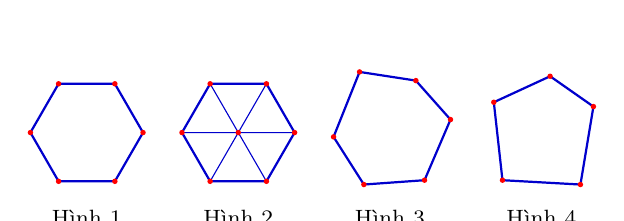
\begin{tikzpicture}[scale=0.55, line cap=round, line join=round]\begin{scope}[xshift=0cm]\foreach \i in {1,...,6} { \coordinate (P\i) at (\i*60:1.3); }\draw[thick, blue!80!black] (P1) -- (P2) -- (P3) -- (P4) -- (P5) -- (P6) -- cycle;\foreach \i in {1,...,6} { \fill[red] (P\i) circle (1.8pt); }\node[below=4pt, font=\footnotesize] at (0,-1.3) {Hình 1};\end{scope}\begin{scope}[xshift=3.5cm]\foreach \i in {1,...,6} { \coordinate (Q\i) at (\i*60:1.3); }\draw[thick, blue!80!black] (Q1) -- (Q2) -- (Q3) -- (Q4) -- (Q5) -- (Q6) -- cycle;\draw[blue!80!black] (Q1)--(Q4) (Q2)--(Q5) (Q3)--(Q6);\foreach \i in {1,...,6} { \fill[red] (Q\i) circle (1.8pt); }\fill[red] (0,0) circle (1.8pt);\node[below=4pt, font=\footnotesize] at (0,-1.3) {Hình 2};\end{scope}\begin{scope}[xshift=7cm]\coordinate (R1) at (1.4,0.3); \coordinate (R2) at (0.6,1.2); \coordinate (R3) at (-0.7,1.4);\coordinate (R4) at (-1.3,-0.1); \coordinate (R5) at (-0.6,-1.2); \coordinate (R6) at (0.8,-1.1);\draw[thick, blue!80!black] (R1) -- (R2) -- (R3) -- (R4) -- (R5) -- (R6) -- cycle;\foreach \p in {R1,R2,R3,R4,R5,R6} { \fill[red] (\p) circle (1.8pt); }\node[below=4pt, font=\footnotesize] at (0,-1.3) {Hình 3};\end{scope}\begin{scope}[xshift=10.5cm]\coordinate (S1) at (1.2,0.6); \coordinate (S2) at (0.2,1.3); \coordinate (S3) at (-1.1,0.7);\coordinate (S4) at (-0.9,-1.1); \coordinate (S5) at (0.9,-1.2);\draw[thick, blue!80!black] (S1) -- (S2) -- (S3) -- (S4) -- (S5) -- cycle;\foreach \p in {S1,S2,S3,S4,S5} { \fill[red] (\p) circle (1.8pt); }\node[below=4pt, font=\footnotesize] at (0,-1.3) {Hình 4};\end{scope}\end{tikzpicture}\end{center}
\choice
{Hình 3}
{Hình 2}
{Hình 1}
{\True Hình 4}
\end{ex}

\begin{ex}
Chọn cách phân tích số $32$ ra thừa số nguyên tố đúng:
\choice
{$32 = 2 \cdot 16$}
{$32 = 8 \cdot 4$}
{\True $32 = 2^5$}
{$32 = 2 \cdot 4 \cdot 4$}
\end{ex}

\begin{ex}
Trong các số sau, số nào chia hết cho cả $2$ và $5$?
\choice
{\True $2020$}
{$25$}
{$52$}
{$5$}
\end{ex}

\begin{ex}
Trong các hình sau, hình nào có hai đường chéo không bằng nhau?
\choice
{Hình chữ nhật}
{Hình thang cân}
{Hình vuông}
{\True Hình bình hành}
\end{ex}

\begin{ex}
\immini{
Nếu có hai miếng bìa hình thang cân với kích thước như hình bên, ta ghép được hình nào sau đây?
\choice
{Hình vuông, hình chữ nhật}
{Hình vuông, hình bình hành}
{\True Hình bình hành, lục giác đều}
{Lục giác đều, hình thang cân}
}{
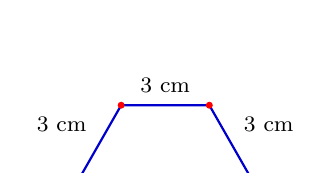
\begin{tikzpicture}[scale=0.7, baseline=(current bounding box.center), line cap=round, line join=round]
  \coordinate (A) at (0.8, 1.4); \coordinate (B) at (2.4, 1.4); \coordinate (C) at (3.2, 0); \coordinate (D) at (0, 0);
  \draw[thick, blue!80!black] (A) -- (B) -- (C) -- (D) -- cycle;
  \foreach \p in {A,B,C,D} \fill[red] (\p) circle (1.8pt);
  \node[above=1pt, font=\footnotesize] at (1.6, 1.4) {$3\text{ cm}$};
  \node[above left=1pt, font=\footnotesize] at (0.4, 0.7) {$3\text{ cm}$};
  \node[above right=1pt, font=\footnotesize] at (2.8, 0.7) {$3\text{ cm}$};
\end{tikzpicture}
}
\end{ex}


\vspace{1mm}
\noindent\textbf{BẢNG TRẢ LỜI TRẮC NGHIỆM PHẦN I:}
\begin{center}
\begin{tabular}{|c|c|c|c|c|c|c|c|c|c|c|c|c|}
\hline
\textbf{Câu} & \textbf{1} & \textbf{2} & \textbf{3} & \textbf{4} & \textbf{5} & \textbf{6} & \textbf{7} & \textbf{8} & \textbf{9} & \textbf{10} & \textbf{11} & \textbf{12} \\
\hline
\textbf{Chọn} & \rule{0pt}{0.65cm} & & & & & & & & & & & \\
\hline
\end{tabular}
\end{center}
\vspace{2mm}

\setcounter{ex}{0}
\noindent\textbf{\large PHẦN II. CÂU TRẮC NGHIỆM ĐÚNG SAI (2,0 điểm)}

\textit{Thí sinh trả lời câu 1 và câu 2. Trong mỗi ý a), b), c), d) ở mỗi câu, thí sinh chọn đúng hoặc sai.}

\vspace{1mm}
\begin{ex}
Xét trong $20$ số tự nhiên đầu tiên (từ $0$ đến $19$). Các khẳng định sau đây đúng hay sai?
\choiceTF
{Trong các số đã cho, có $3$ số chia hết cho cả $2$ và $5$}
{Trong các số đã cho, có $6$ số chia hết cho $9$}
{\True Trong các số đã cho, có $8$ số là số nguyên tố}
{Trong các số đã cho, có $6$ số là bội của $3$}
\end{ex}

\begin{ex}
Xét việc phân tích số $40$ ra thừa số nguyên tố. Các khẳng định sau đây đúng hay sai?
\choiceTF
{\True Phân tích số $40$ ra thừa số nguyên tố ta được kết quả là $40 = 2^3 \cdot 5$}
{Kết quả phân tích số $40$ ra thừa số nguyên tố là $40 = 4 \cdot 10$}
{Kết quả phân tích số $40$ ra thừa số nguyên tố là $40 = 2 \cdot 4 \cdot 5$}
{Số $40$ có tất cả $3$ thừa số nguyên tố khác nhau là $2, 3$ và $5$}
\end{ex}


\noindent\textbf{BẢNG TRẢ LỜI PHẦN II:}
\begin{center}
\begin{tabular}{|c|c|c|c|c||c|c|c|c|c|}
\hline
\textbf{Câu 1} & \textbf{a)} & \textbf{b)} & \textbf{c)} & \textbf{d)} & \textbf{Câu 2} & \textbf{a)} & \textbf{b)} & \textbf{c)} & \textbf{d)} \\
\hline
\textbf{Đ/S} & \rule{0pt}{0.6cm} & & & & \textbf{Đ/S} & & & & \\
\hline
\end{tabular}
\end{center}
\vspace{2mm}

\setcounter{ex}{0}
\noindent\textbf{\large PHẦN III. CÂU HỎI TRẢ LỜI NGẮN (2,0 điểm)}

\textit{Thí sinh trả lời câu 1 và câu 2. Điền kết quả số vào ô trống tương ứng.}

\vspace{1mm}
\begin{ex}
Có bao nhiêu số tự nhiên $m$ sao cho $5 < m < 15$ và $m \ \vdots \ 3$? \shortans{$3$}
\end{ex}

\begin{ex}
Tìm số tự nhiên $x$ lớn nhất thỏa mãn $120 \ \vdots \ x$ và $150 \ \vdots \ x$. \shortans{$30$}
\end{ex}


\setcounter{ex}{0}
\noindent\textbf{\large PHẦN IV. TỰ LUẬN (3,0 điểm)}

\textit{Thí sinh trình bày chi tiết lời giải vào giấy làm bài.}

\vspace{1mm}
\begin{ex} (1.0 điểm)
Thực hiện phép tính (tính hợp lí nếu có thể):
\begin{enumerate}[label=\textbf{\alph*)}, leftmargin=0.8cm, itemsep=2pt]
\item $3^4 : 3^2$
\item $80 - (4 \cdot 5^2 - 3 \cdot 2^3)$
\item $23 \cdot 75 + 25 \cdot 10 + 25 \cdot 13$
\end{enumerate}
\end{ex}
\vspace{1.5mm}

\begin{ex} (0.75 điểm)
Tìm số tự nhiên $x$, biết:
\begin{enumerate}[label=\textbf{\alph*)}, leftmargin=0.8cm, itemsep=2pt]
\item $120 - 5(x + 2) = 20$
\item $x \ \vdots \ 20$, $x \ \vdots \ 35$ và $400 < x < 500$
\end{enumerate}
\end{ex}
\vspace{1.5mm}

\begin{ex} (0.75 điểm)
Cô giáo chủ nhiệm muốn chia $72$ quyển vở, $48$ bút bi và $60$ gói bánh thành một số phần thưởng như nhau để trao trong dịp sơ kết học kì.
\begin{enumerate}[label=\textbf{\alph*)}, leftmargin=0.8cm, itemsep=2pt]
\item Hỏi có thể chia được nhiều nhất bao nhiêu phần thưởng?
\item Khi đó mỗi phần thưởng có bao nhiêu quyển vở, bút bi và gói bánh?
\end{enumerate}
\end{ex}
\vspace{1.5mm}

\begin{ex} (0.5 điểm)
\begin{enumerate}[label=\textbf{\alph*)}, leftmargin=0.8cm, itemsep=2pt]
\item Cho số tự nhiên $x$ thỏa mãn $3^{x+1} + 3^{x+2} - 2 \cdot 3^x = 270$. Hỏi $x$ là số nguyên tố hay hợp số?
\item Tìm hai số tự nhiên biết tích của chúng bằng $144$ và ước chung lớn nhất của chúng bằng $6$.
\end{enumerate}
\end{ex}
\vspace{1.5mm}


\begin{center}
\rule{4cm}{0.4pt}\\
\textit{--- HẾT ---}
\end{center}
\end{document}
